% =====================================================================
%  Chapter 1 -- Introduction
% =====================================================================
\chapter{Introduction}\label{ch:intro}
\chapterlists[f]

\section{Tipping points}\label{sec:tipping}

Lean back slowly on a chair. For a while every small push produces a small tilt and the chair comes
back; then, at one angle, the same push sends it to the floor. A \emph{tipping point} is such a
condition: a small change in circumstances produces a large and often lasting change of state.
Retreating ice sheets, dying-back forests and a weakening ocean circulation have all been described in
these terms~\cite{Lenton2008}. This report concerns one cause of tipping that is easy to state and
hard to observe: a system can tip simply because its surroundings change \emph{too fast}.

\section{Three routes to tipping}\label{sec:three-routes}

Picture a stable state as a ball at the bottom of a valley. The ball is the state of the system; the
landscape is set by a parameter $\mu$. Ashwin \emph{et al.}~\cite{Ashwin2012} distinguished three
ways in which the ball can leave its valley (\cref{fig:tipping-types}).

\begin{figure}[!htb]
  \centering
  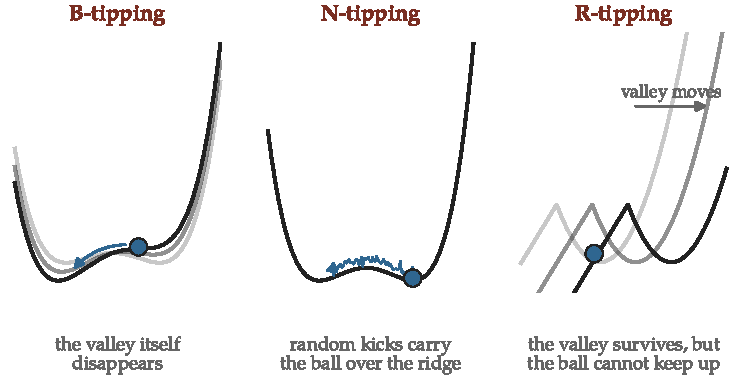
\includegraphics[width=\linewidth]{fig_tipping_types}
  \caption[Three routes to tipping]{Three routes to tipping. B: the valley vanishes as the parameter
  passes a critical value. N: random kicks carry the ball over the ridge. R: the valley keeps its shape
  but moves so quickly that the ball is left behind.}
  \label{fig:tipping-types}
\end{figure}

\begin{itemize}
  \item \textbf{Bifurcation-induced (B-tipping).} The parameter passes a critical value at which the
        stable state disappears. What matters is \emph{where} the parameter is.
  \item \textbf{Noise-induced (N-tipping).} Random disturbances push the system over a barrier in a
        fixed landscape. What matters is \emph{how noisy} the system is.
  \item \textbf{Rate-induced (R-tipping).} The stable state always exists, but it moves faster than
        the system can follow. What matters is \emph{how fast} the parameter changes.
\end{itemize}
R-tipping, the subject of this report, is the least intuitive: at every instant a perfectly good stable
state is available, yet the system fails to keep up with it.

\section{Rate-induced tipping in two lines of mathematics}\label{sec:rtip-maths}

Let a state $x$ evolve under a parameter $\mu$ that changes at a constant rate $r$,
\begin{equation}
  \dot{x} = f\bigl(x,\mu(t)\bigr), \qquad \mu(t) = r\,t .
  \label{eq:nonautonomous}
\end{equation}
For frozen $\mu$ the system would rest at a stable state $x^{*}(\mu)$, defined by
\begin{equation}
  f\bigl(x^{*}(\mu),\mu\bigr) = 0 .
  \label{eq:frozen-state}
\end{equation}
Writing $y = x - x^{*}(\mu(t))$ for the lag behind this moving target and differentiating,
\begin{equation}
  \dot{y} \;=\; f\bigl(x^{*}+y,\mu\bigr) \;-\; r\,\frac{\dd x^{*}}{\dd\mu} .
  \label{eq:moving-frame}
\end{equation}

\begin{whybox}[Reading \cref{eq:moving-frame}]
The first term pulls the lag back towards zero. The second is a drag, proportional to $r$, that exists
only because the stable state moves. For small $r$ the pull wins and the lag settles; for large $r$ the
drag wins and the system tips. The boundary is the \emph{critical rate} $r_{c}$.
\end{whybox}

A minimal example makes this concrete:
\begin{equation}
  \dot{x} = 1 - (x-\mu)^{2}, \qquad \dot{\mu} = r .
  \label{eq:toy-model}
\end{equation}
For any frozen $\mu$ it has a stable state $x^{*}=\mu+1$ and an unstable one (the ridge) at
$x=\mu-1$; no bifurcation ever occurs. In the moving frame $y=x-\mu$,
\begin{equation}
  \dot{y} = 1 - r - y^{2} ,
  \label{eq:toy-moving}
\end{equation}
which has a stable steady lag $y=\sqrt{1-r}$ only if
\begin{equation}
  r < r_{c} = 1 .
  \label{eq:toy-rc}
\end{equation}
Above $r_{c}$ the state escapes across the ridge (\cref{fig:rate-tracking}). The parameter follows the
same path in both panels of the figure; only the speed differs, and the speed alone decides the outcome.

\begin{figure}[!htb]
  \centering
  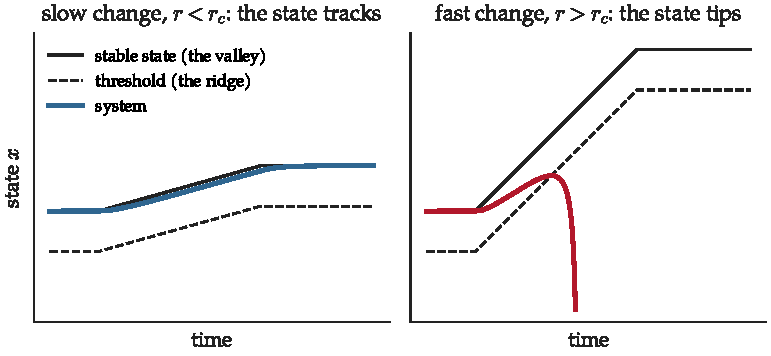
\includegraphics[width=\linewidth]{fig_rate_tracking}
  \caption[Tracking and tipping in a minimal model]{The model of \cref{eq:toy-model}, ramped over the
  same range and then held. Left: $r<r_{c}$, the state tracks its moving stable state. Right: $r>r_{c}$,
  the state falls behind, crosses the moving threshold and tips.}
  \label{fig:rate-tracking}
\end{figure}

R-tipping has been studied extensively in models of natural and human
systems~\cite{Ritchie2023,Wieczorek2023}; controlled laboratory demonstrations remain
rare~\cite{Tony2017}.

\section{What would convince us? Three criteria}\label{sec:criteria}

We set three criteria for a convincing demonstration, each illustrated by carrying a full cup of coffee
across a room. The cup is the parameter we control; the coffee is the system.

\paragraph{Criterion 1: the system lags behind a moving threshold}
When the cup starts to move, the coffee surface tilts backwards: it responds to where the cup
\emph{was}, not where it is. In the circuit, the oscillation should switch on at a gain \emph{above}
threshold when the gain rises, and switch off \emph{below} threshold when it falls, so that an up-down
sweep traces a loop.

\paragraph{Criterion 2: the lag grows with the rate in a predictable way}
Walk faster and the coffee tilts more, by an amount that physics predicts. A lag alone proves little,
since any instrument has delays; a fixed instrumental delay shifts the threshold in proportion to the
rate. The dynamics near an instability predict a different law: in our circuit, a displacement
a shift of the switching resistance $\propto\sqrt{\lambda}$, where $\lambda$ is the sweep rate, with a coefficient fixed by the components (\cref{ch:theory}).

\paragraph{Criterion 3: the long-time state depends on the rate alone}
Carry the cup along the same route a little too briskly and the coffee spills, for good. The route is
identical; the speed decides the final state. In the circuit, we sweep the gain along one fixed path,
again and again, varying only the speed. Below a critical rate the oscillation should return every
cycle; above it, it should vanish and stay away, although the gain keeps crossing the threshold.
Criteria 1 and 2 are addressed in \cref{ch:stage1,ch:stage2,ch:stage3}, Criterion 3 in
\cref{ch:stage4}, and all three are reviewed in \cref{ch:discussion}.

\section{Why an electronic oscillator}\label{sec:outline}

Natural systems that tip cannot be reset, their parameters cannot be dialled, and one ``run'' may take
decades. In a Wien-bridge oscillator the distance from threshold is set by a single resistor that a
microcontroller can move along any path at any speed; the circuit runs at about \SI{73}{\hertz}, so a
sweep cycle lasts seconds; it obeys a second-order linear equation until the amplifier saturates, so
predictions are quantitative; and it can be simulated at component level.

\begin{figure}[!htb]
\centering
\begin{tikzpicture}[
    stage/.style={draw=accent, line width=0.6pt, rounded corners=3pt, fill=boxbg, text width=3.05cm,
                  minimum height=2.3cm, align=left, inner sep=6pt, font=\footnotesize},
    arr/.style={-{Stealth[length=2.2mm]}, line width=0.7pt, color=soft}]
  \node[stage] (s1) {\textbf{Stage 1}\\[1pt] \emph{Simulation, smooth ramp}\\[3pt] Does the circuit lag,
        and how does the lag scale?};
  \node[stage, right=0.42cm of s1] (s2) {\textbf{Stage 2}\\[1pt] \emph{Bench, staircase in $\RF$}\\[3pt]
        Does real hardware obey the same law?};
  \node[stage, right=0.42cm of s2] (s3) {\textbf{Stage 3}\\[1pt] \emph{Simulation, staircase in $\RF$}\\[3pt]
        What happens beyond bench rates?};
  \node[stage, right=0.42cm of s3, fill=keybg, draw=ink] (s4) {\textbf{Stage 4}\\[1pt] \emph{Bench and
        simulation, staircase in $\Ri$}\\[3pt] Does the final state depend on speed alone?};
  \draw[arr] (s1) -- (s2); \draw[arr] (s2) -- (s3); \draw[arr] (s3) -- (s4);
\end{tikzpicture}
\caption[The four stages of the project]{The four stages of the project; each answered one question and
raised the next.}
\label{fig:roadmap}
\end{figure}

The report follows the four stages of \cref{fig:roadmap}. \Cref{ch:theory} develops the theory,
\cref{ch:methods} the methods, \cref{ch:stage1,ch:stage2,ch:stage3,ch:stage4} the four stages,
\cref{ch:discussion} the discussion, and \cref{ch:conclusion} the conclusion and outlook.
